\chapter{Execução do Estudo de Caso e Análise dos Dados}
\label{chap:execucao}

Neste capítulo serão apresentadas as análises dos dados quantitativos e qualitativos e a discussão dos resultados.


\section{Analise do SIGET}

Para cada uma das \textit{releases} do SIGET, coletou-se o código-fonte, conforme a disponibilidade, no repositório da CAIXA. Após a obtenção do código-fonte,foi realizado a análise estática cada \textit{release} utilizando as ferramentas analizo, findbugs e PMD. Posteriormente, os resultados das análises foram extraídos, transformados e carregados no ambiente de Data Warehousing proposto no Capítulo \ref{chap:arquitetura}. Dessa forma, foi possível obter:

\begin{easylist}[itemize]

& O intervalo qualitativo para cada uma das Métricas de Código-Fonte por \textit{index} e por \textit{release}; 

& Quantidade de Cenários de Limpeza total, por tipo e por \textit{release}; 

& Classe, nome e recomendação para cada cenário de limpeza; 

& Quantidade de \textit{bugs} total,por tipo, por \textit{index} e por \textit{release};

& Classe, tipo, nome e linha para cada \textit{bug}; 

& Quantidade de violações total,por tipo, por \textit{index} e por \textit{release};

& Classe, tipo, nome e linha para cada violação; 

\end{easylist}

Como demonstrado nas Figuras \ref{dashboardtotal}, \ref{dashboardPMD}, \ref{dashboardFindbugs} e \ref{dashboardCenarios}.

\begin{figure}[h!]
\centering
\includegraphics[keepaspectratio=false,scale=0.4]{figuras/figuras_nilton/DashboardTotal.eps}
\caption{\textit{Dashboard} Quantidade Total}
\label{dashboardtotal}
\end{figure}

\begin{figure}[h!]
\centering
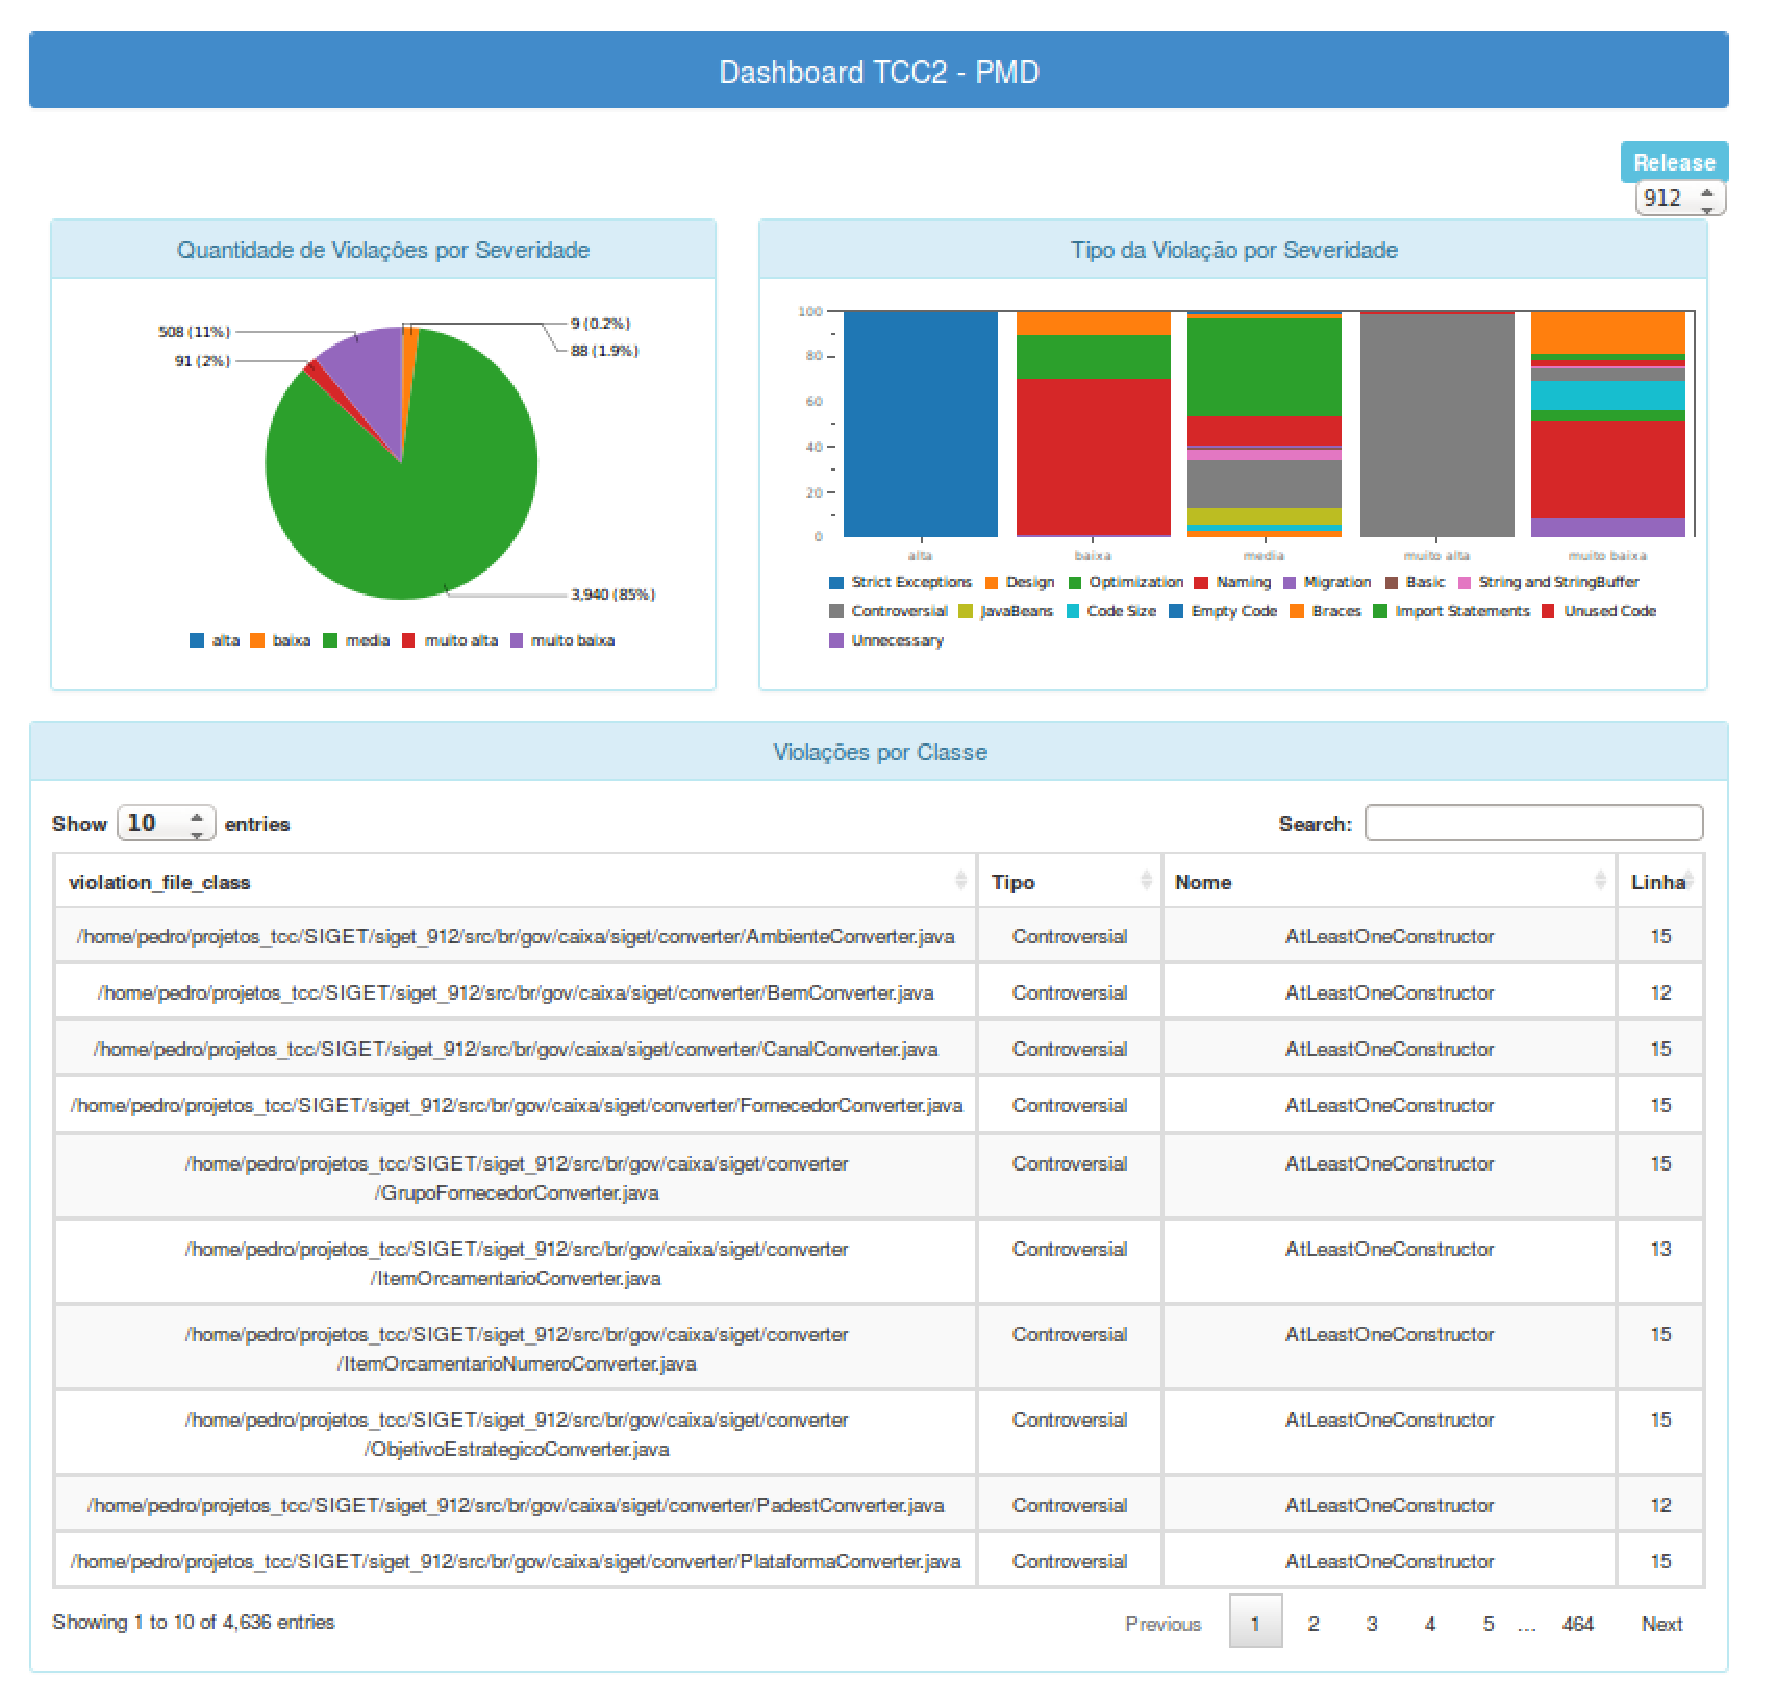
\includegraphics[keepaspectratio=false,scale=0.5]{figuras/figuras_nilton/DashboardPMD.eps}
\caption{\textit{Dashboard PMD}}
\label{dashboardPMD}
\end{figure}

\begin{figure}[h!]
\centering
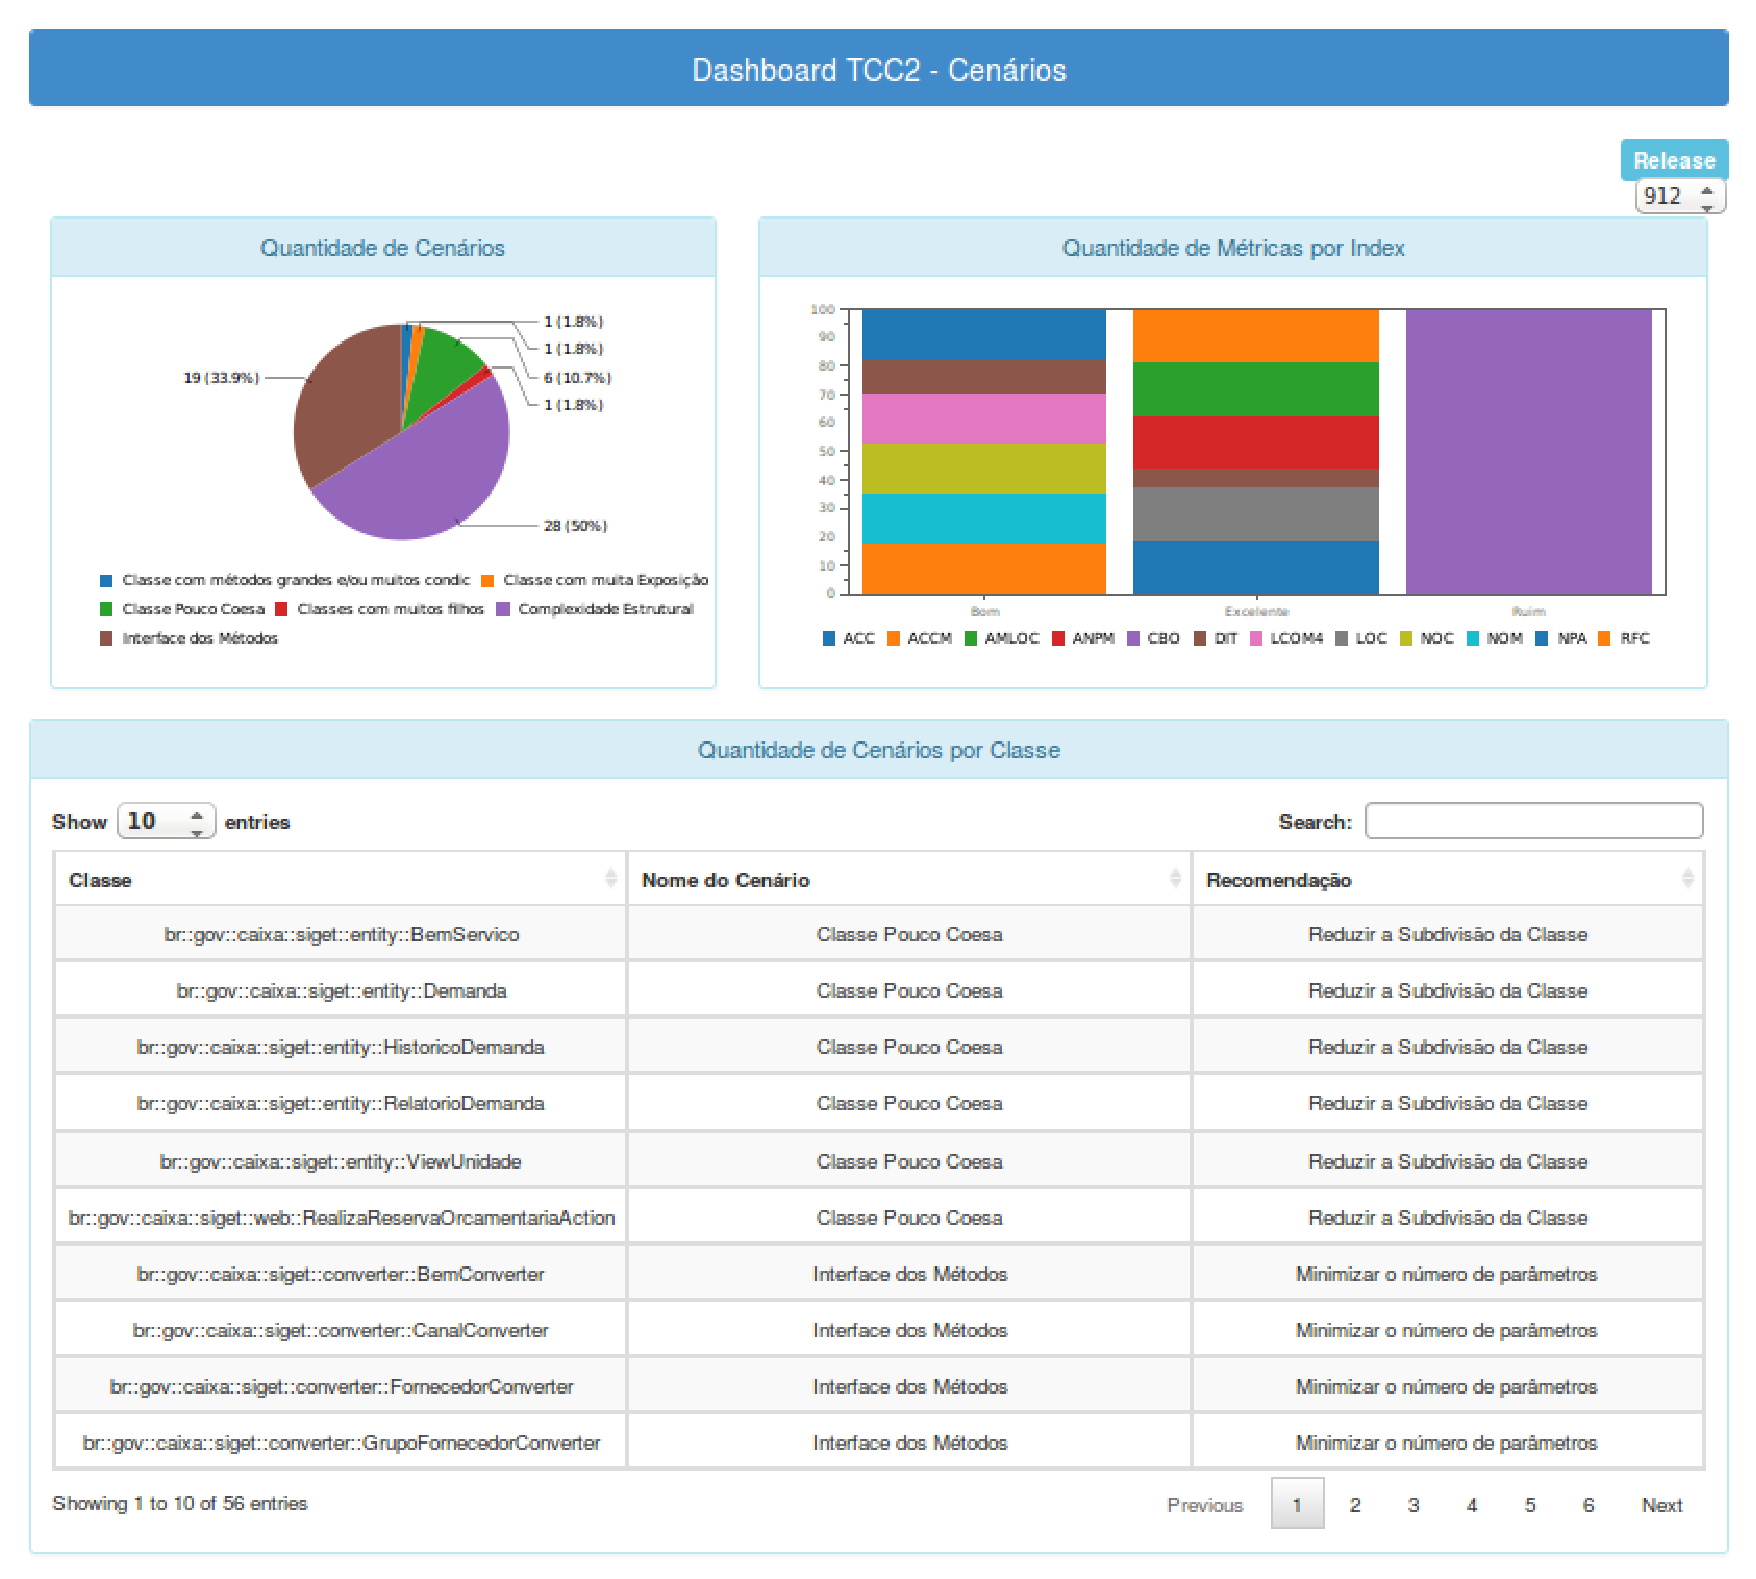
\includegraphics[keepaspectratio=false,scale=0.5]{figuras/figuras_nilton/DashboardCenarios.eps}
\caption{\textit{Dashboard} Cenários}
\label{dashboardFindbugs}
\end{figure}

\begin{figure}[h!]
\centering
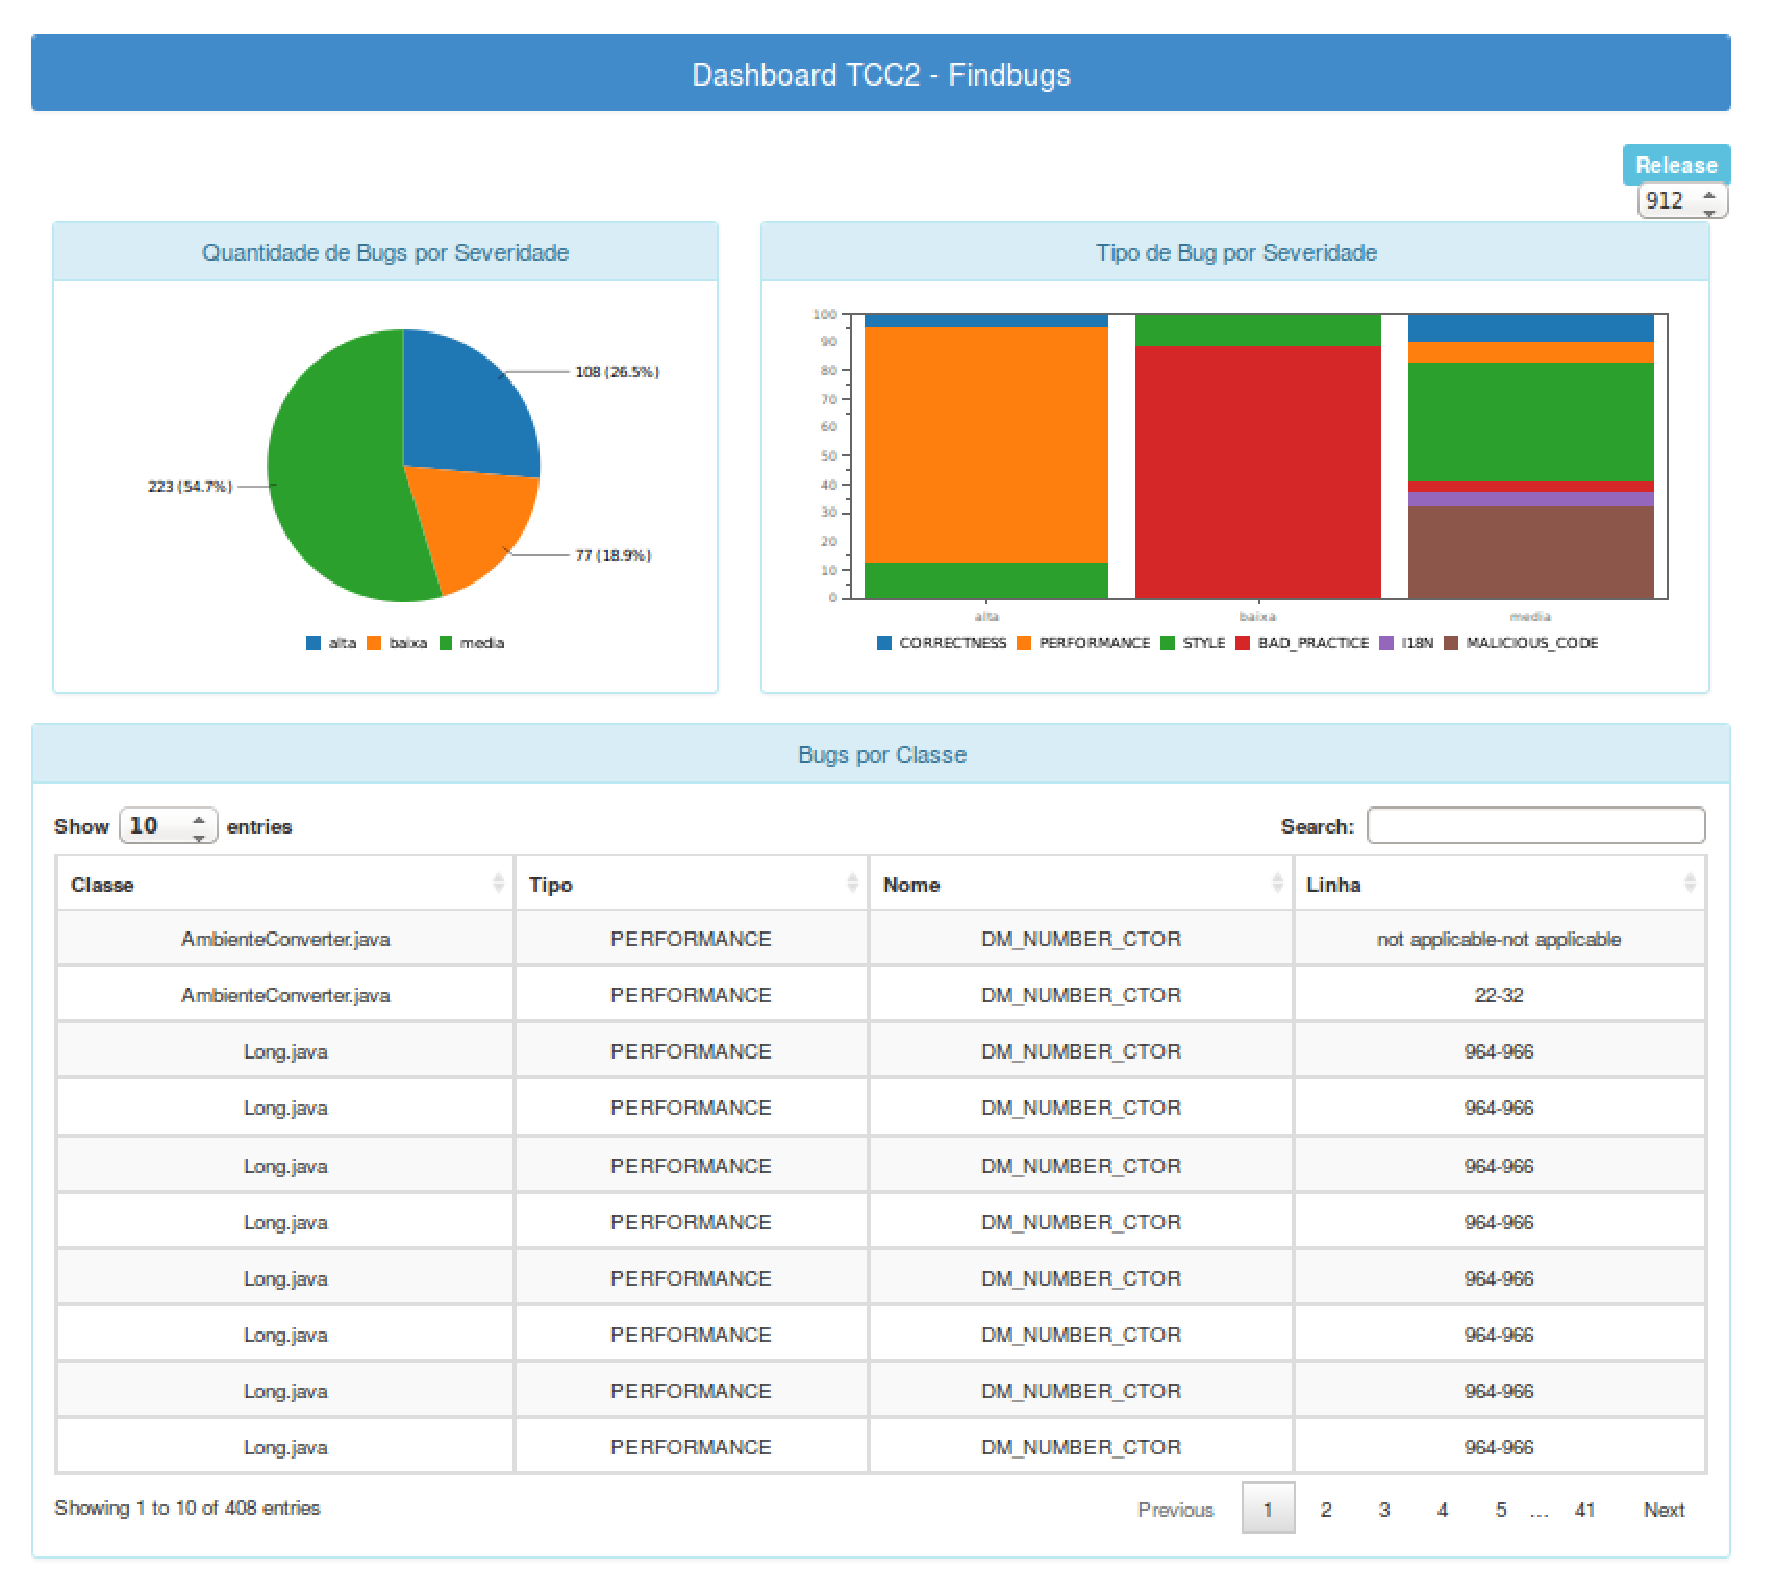
\includegraphics[keepaspectratio=false,scale=0.5]{figuras/figuras_nilton/DashboardFindbugs.eps}
\caption{\textit{Dashboard FindBugs}}
\label{dashboardCenarios}
\end{figure}

\section{Analise do Questionário}



\section{Analise do Erro Quadrático Médio}

Com o objetivo de validar a corretude dos dados apresentados pela solução de DW foi realizado o calculo do EQM (Erro Quadrático Médio). EQM é a soma das diferenças entre
o valor estimado e o valor real dos dados, ponderados pelo número de termos: 

$ EQM = \sum\limits_{i}\frac{(x{i}-y{i})^{2}}{n} $

Quanto mais próximo o valor do EQM de 0, maior a corretude e menor é a diferença entre os valores estimados e os valores reais.

Tomando como referência o valor estimado como os valores apresentados pela a solução de DW e o valor real como os valores apresentados pelas ferramentas \textit{FindBugs} e PMD utilizadas individualmente. Foi calculado o EQM de cada conjunto de regra do FindBugs e do PMD de todas as \textit{releases}, as Figuras \ref{EQMFindBugs}, \ref{EQMPMD1}, \ref{EQMPMD2} e \ref{EQMPMD3} mostram os resultados do EQM. Os valores apresentados pelas ferramentas utilizadas individualmente foram coletados de arquivos do tipo csv por elas geradas, que estão disponíveis para consulta no repositório deste trabalho no \textit{github} \footnote{https://github.com/NiltonAraruna/}. Os valores da solução de DW foram coletados a partir dos \textit{Dashboards} da própria solução.

\begin{figure}[h!]
\centering
\includegraphics[keepaspectratio=false,scale=0.45,angle=90]{figuras/figuras_nilton/EQMFindBugs.eps}
\caption{\textit{Resultados do EQM do FindBugs}}
\label{EQMFindBugs}
\end{figure}

\begin{figure}[h!]
\centering
\includegraphics[keepaspectratio=false,scale=0.45,angle=90]{figuras/figuras_nilton/EQMPMD1.eps}
\caption{\textit{Resultados do EQM do PMD}}
\label{EQMPMD1}
\end{figure}

\begin{figure}[h!]
\centering
\includegraphics[keepaspectratio=false,scale=0.45,angle=90]{figuras/figuras_nilton/EQMPMD2.eps}
\caption{\textit{Continuação Resultados do EQM do PMD}}
\label{EQMPMD2}
\end{figure}

\begin{figure}[h!]
\centering
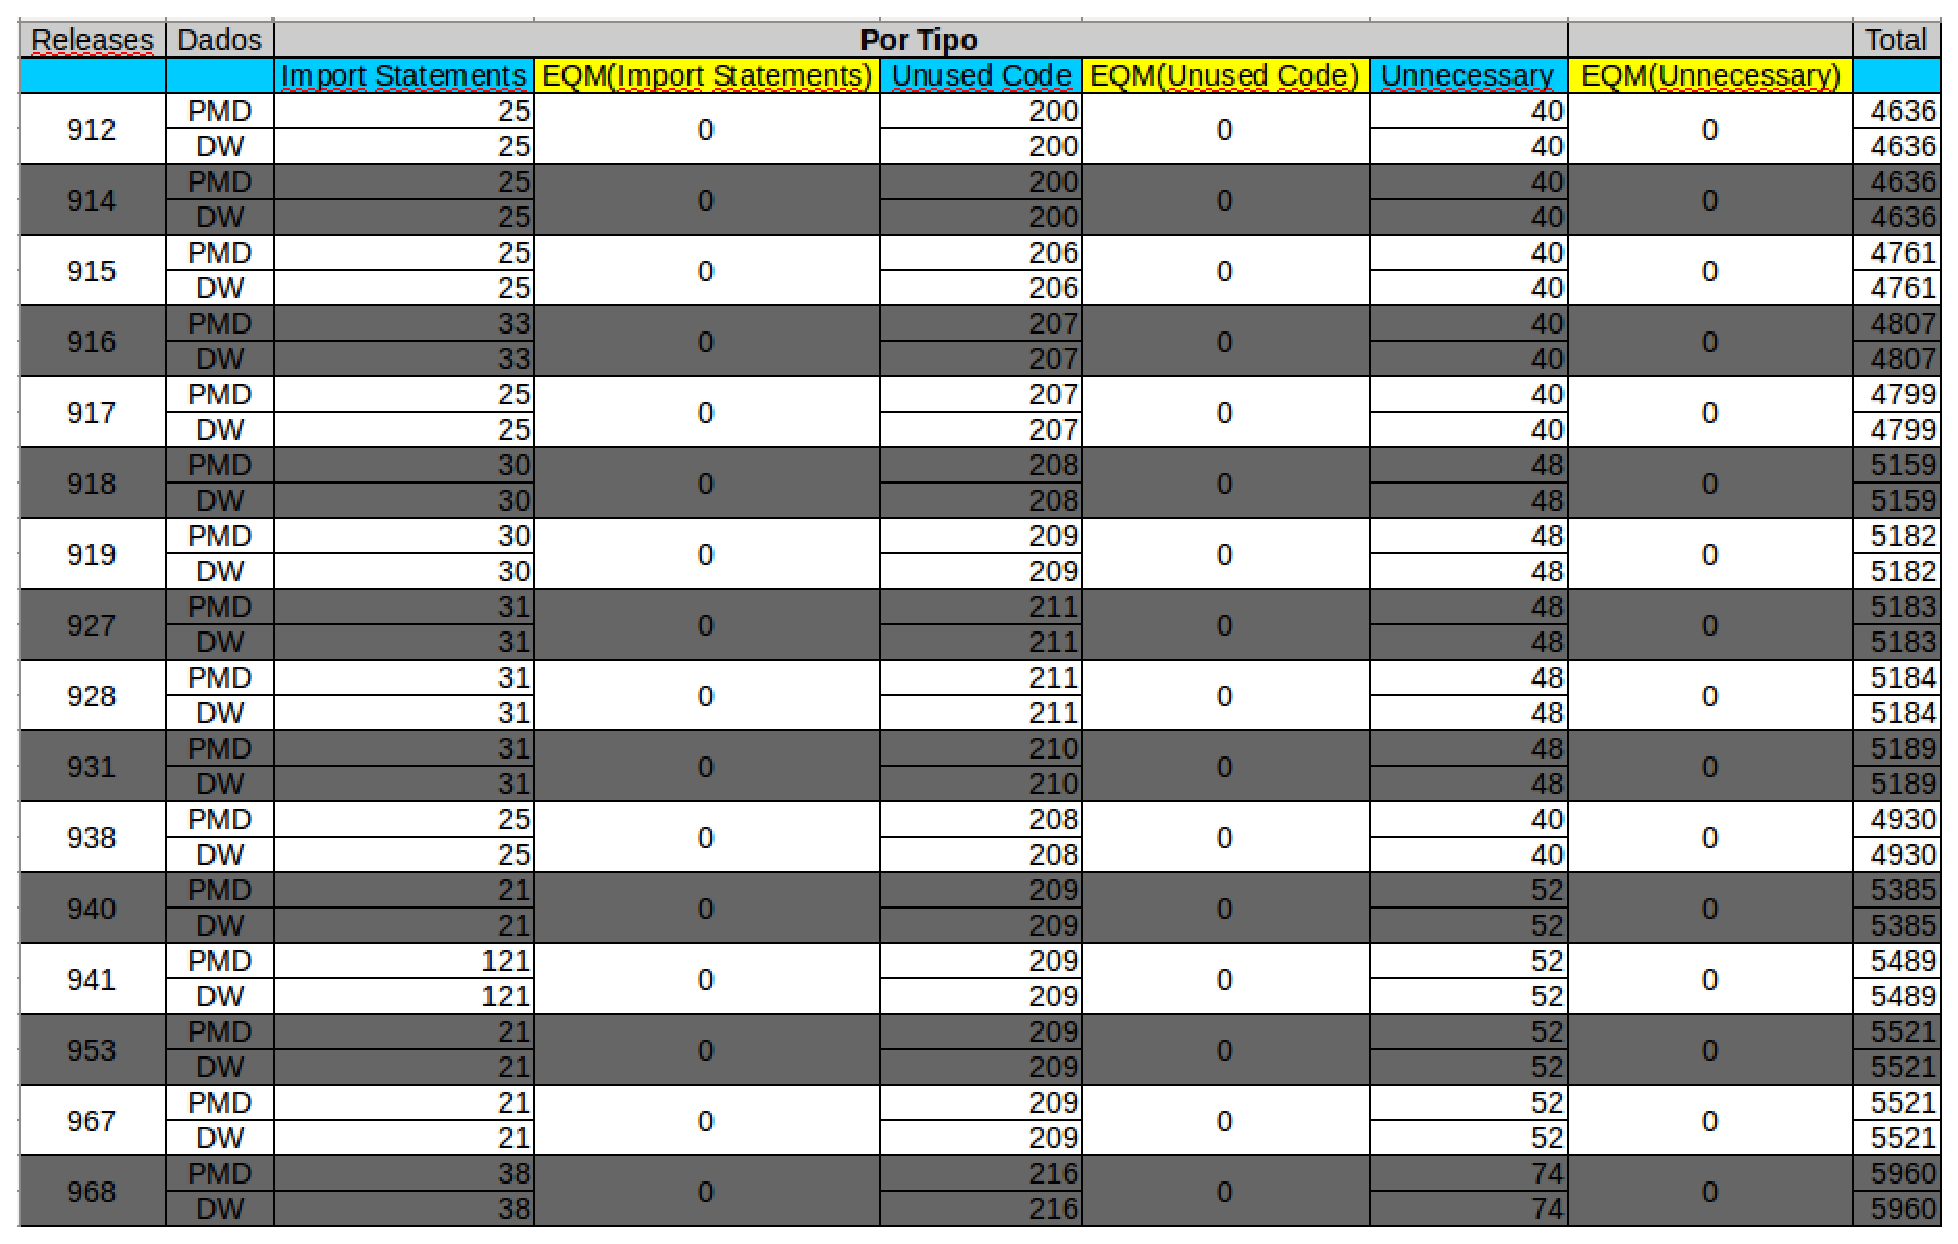
\includegraphics[keepaspectratio=false,scale=0.45,angle=90]{figuras/figuras_nilton/EQMPMD3.eps}
\caption{\textit{Continuação Resultados do EQM do PMD}}
\label{EQMPMD3}
\end{figure}

Como pode ser observado os resultados obtidos do EQM foram todos igual a 0, significando a corretude entre os valores obtidos através do \textit{FindBugs} e PMD e os valores apresentados pela solução de DW. A corretude dos valores dos cenários de limpeza não foram validados porque algumas correções e adaptações tiveram que ser feitas na solução de DW de \cite{rego_monitoramento_2014} para que possibilitasse as análises do SIGET, como a adição das função \textit{ROUND} no step "Inserindo os Fatos na $F_Project_Metric $" da transformação "Percentiles Analizo".  


\section{Analise do Coeficiente de Correlação}

Segundo \cite{Wasserman2010}, o coeficiente de correlação linear r, proposto por Karl Pearson, é calculado a partir de uma amostra de n pares de observações de X e Y, e mede a intensidade e a direção da relação linear entre duas variáveis quantitativas e o grau de correlação entre as variáveis:

$ r = \frac{\sum(X-X')(Y-Y')}{\sqrt{[\sum(X-X')^{2}][\sum(Y-Y')^{2}]}} $


Correlação entre duas variáveis é quando uma delas está, de alguma forma, relacionada com a outra. A Tabela \ref{tab:correlacao} mostra a significância de índice de Correlação segundo \cite{Wasserman2010}.

\begin{table}[!ht]
	\begin{center}
\input{tabelas/tabelasNilton/correlacao.ltx} 
	\caption{Significância de índice de Correlação}
	\label{tab:correlacao}
	\end{center}
	\end{table}	
	\FloatBarrier

Um diagrama de dispersão também demostra a relação entre duas variáveis quantitativas, medidas sobre os mesmos indivíduos. Se a reta do gráfico for mais próxima de
uma reta de 45 graus, maior será a correlação positiva, se a reta apresentada for mais próxima de 135 graus, maior será a correlação negativa. 

Não querendo generalizar o resultado de uma possível correlação entre \textit{bugs}, violações e cenários de limpeza por se tratar de um estudo de apenas um estudo de caso, uma instituição e um sistema foi calculado o coeficiente de correlação linear entre \textit{bugs} e violações, entre \textit{bugs} e cenários de limpeza e entre cenários de limpeza e violações. O resultado do cálculo do coeficiente de correlação linear pode ser vista na Figura \ref{correlacao}.

\begin{figure}[h!]
\centering
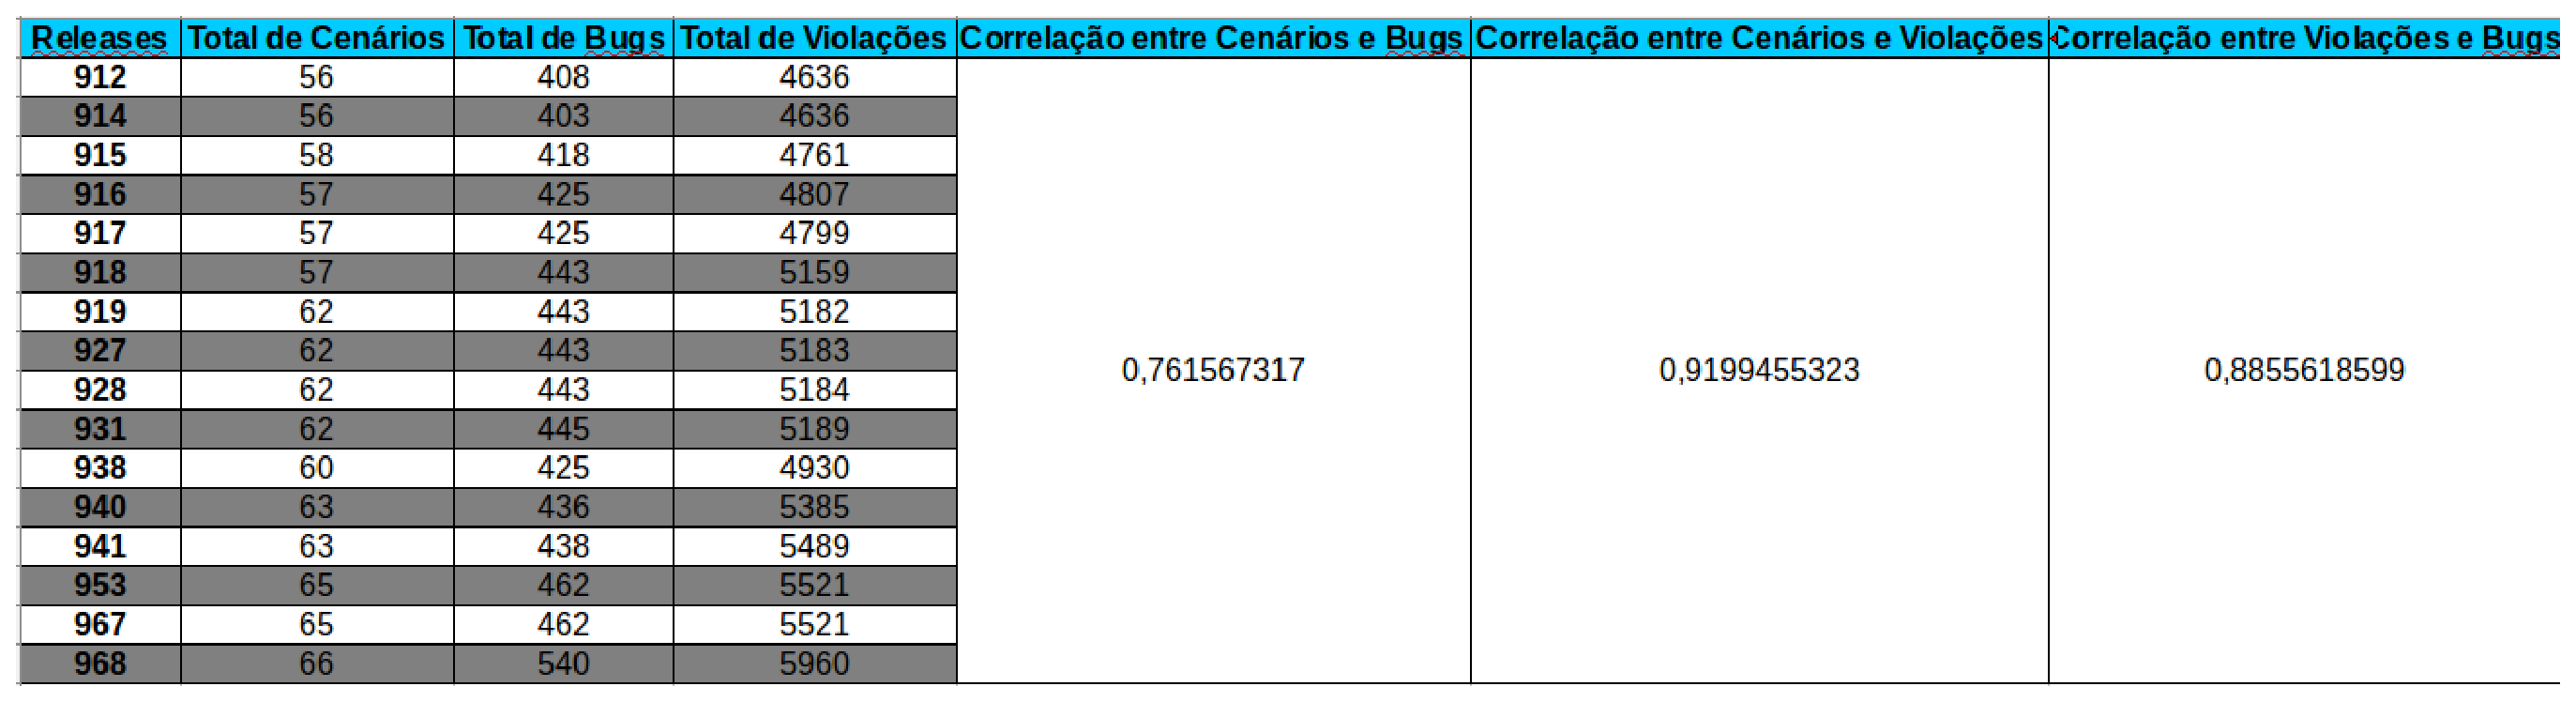
\includegraphics[keepaspectratio=false,scale=0.40,angle=90]{figuras/figuras_nilton/correlacao.eps}
\caption{Resultado do cálculo do coeficiente de correlação linear}
\label{correlacao}
\end{figure}

Analisando os resultados do coeficiente de correlação linear em conformidade com a Tabela \ref{tab:correlacao} podemos notar que a correlação entre cenários de limpeza e violações, entre violações e \textit{bugs} e correlação entre cenários e \textit{bugs} é uma correlação direta e muito forte. Os gráficos de dispersão das Figuras \ref{dispercaocenariosbugs}, \ref{dispersaocenariosviolacoes} e \ref{dispersaoviolacoesbugs} também demonstra uma correlação direta e muito forte pois as retas dos gráficos se aproximam de 45 graus.

\begin{figure}[h!]
\centering
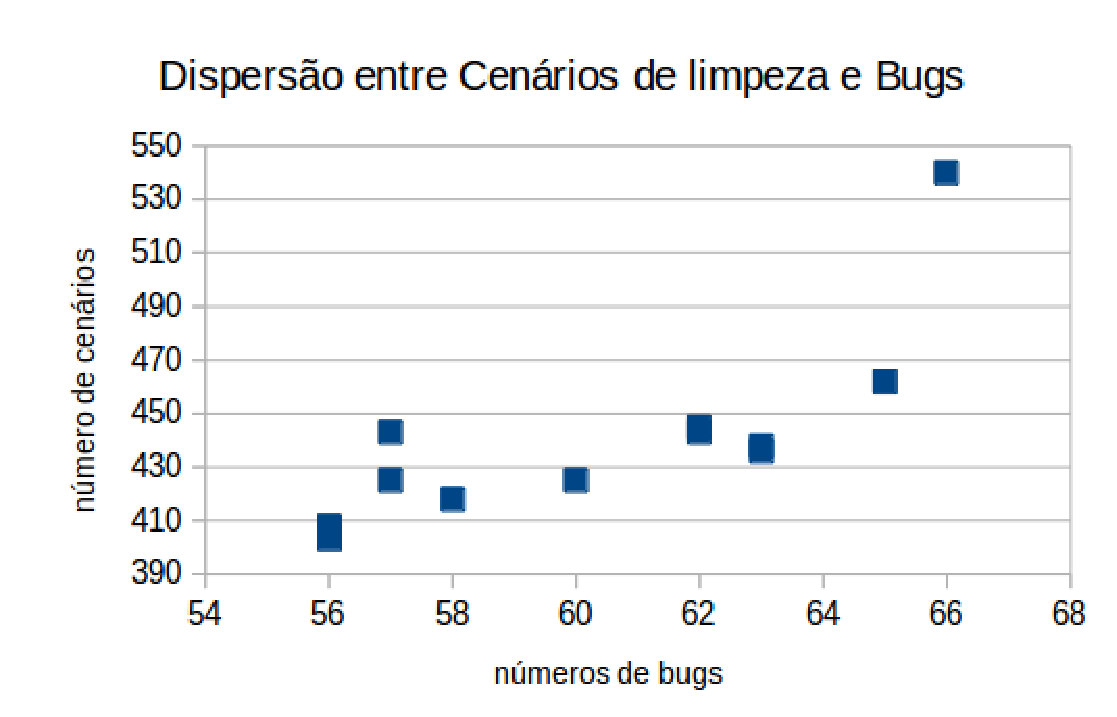
\includegraphics[keepaspectratio=false,scale=0.40]{figuras/figuras_nilton/dispercaocenariosbugs.eps}
\caption{Gráfico de Dispersão entre Cenários de Limpeza e \textit{Bugs}}
\label{dispercaocenariosbugs}
\end{figure}


\begin{figure}[h!]
\centering
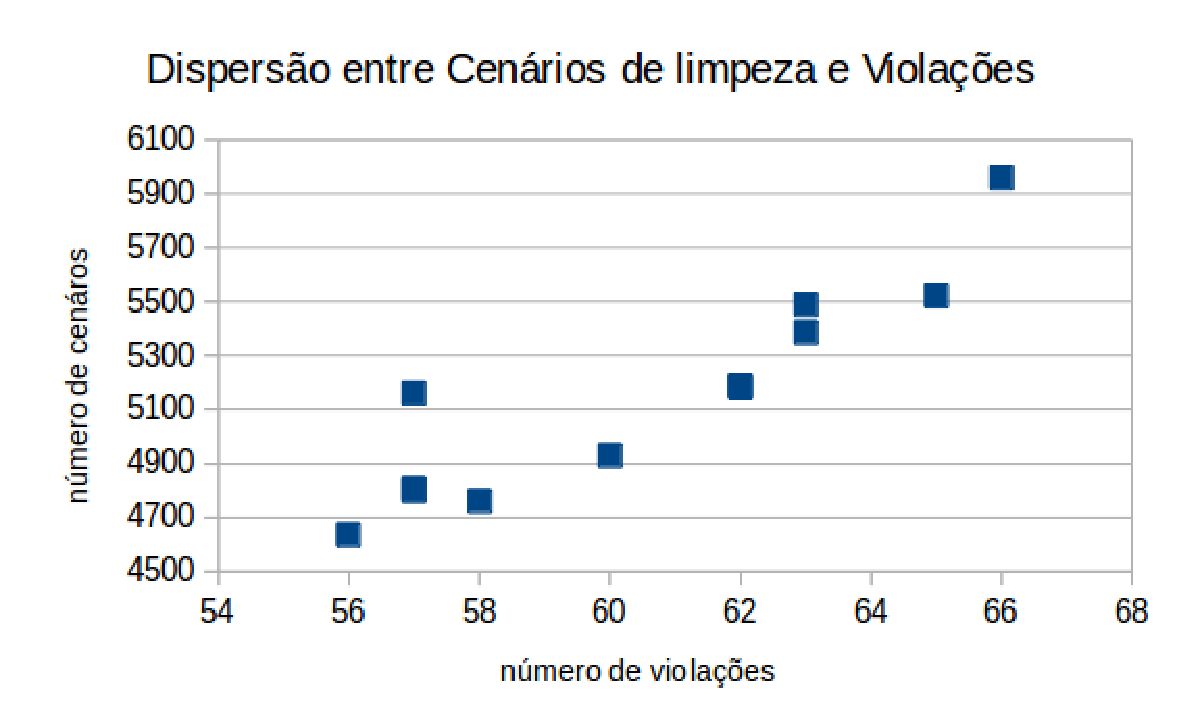
\includegraphics[keepaspectratio=false,scale=0.40]{figuras/figuras_nilton/dispersaocenariosviolacoes.eps}
\caption{Gráfico de Dispersão entre Cenários de Limpeza e Violações}
\label{dispersaocenariosviolacoes}
\end{figure}

\begin{figure}[h!]
\centering
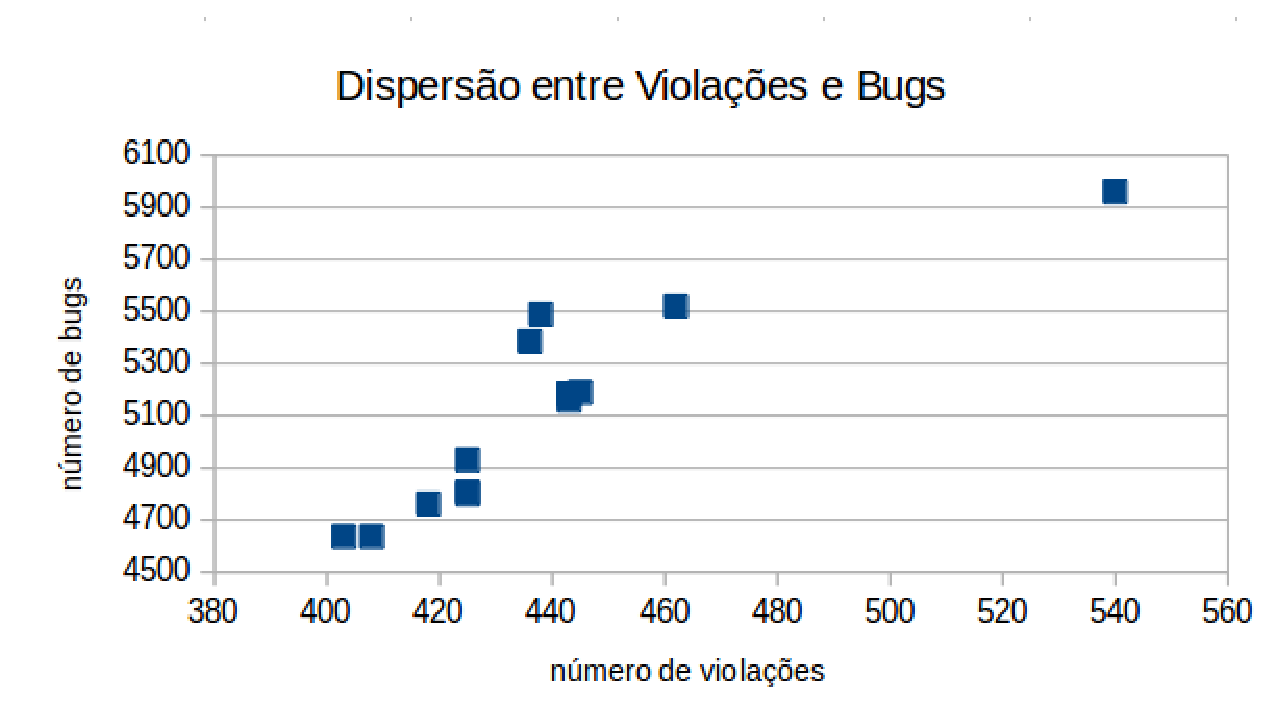
\includegraphics[keepaspectratio=false,scale=0.40]{figuras/figuras_nilton/dispersaoviolacoesbugs.eps}
\caption{Gráfico de Dispersão entre Violações e \textit{Bugs}}
\label{dispersaoviolacoesbugs}
\end{figure}